\pdfminorversion=6 % this is needed to be able to include pdf 1.6. 
                    % For some reasons some old HPSG proceedings have pdf 1.6
\documentclass[11pt,a4paper,fleqn]{article}
\usepackage{times}
\thispagestyle{empty}



\usepackage[T1]{fontenc}   % Silbentrennung

\usepackage[utf8x]{inputenc}
                                                                                                                             
\hyphenation{Acad-e-my}

\usepackage[bookmarks=true,bookmarksopen=true,%
breaklinks=true,%
draft=false,plainpages=false,hyperfootnotes=false,%
pdfauthor={Stefan  Müller, Petya Osenova (Editors)},%
pdftitle={Proceedings of the 26th International Conference on Head-Driven Phrase Structure Grammar},%
pdfkeywords={HPSG}%,
pdftex=true%
%ps2pdf=true  %ohne diesen Treiber geht der Zeilenumbruch in URLs
]{hyperref}% for pdf files
\hypersetup{colorlinks=false, pdfborder={0 0 0}}

\usepackage{pdfpages}
\pdfinclusioncopyfonts=1

\newcommand\formatauthor[2]{\begin{tabular}[t]{@{}c@{}}
  {\LARGE#1\strut}\\
  {\small#2\strut}\\
  \rule{\dimexpr0.5\linewidth-1em}{0pt}
  \end{tabular}\xhfill\ignorespaces}
\newcommand\xhfill{\hspace{1em plus 1fill}}

\begin{document}

\begin{center}
{\Large
                {\bfseries Proceedings of the 26th International Conference on\par Head-Driven Phrase Structure Grammar\par}

                \vspace{8ex}

                     University of Bucharest\\[\baselineskip]

                        Stefan  M{\"u}ller, Petya Osenova (Editors)\\[\baselineskip]

                                2019\\[\baselineskip]

                          CSLI Publications\\[\baselineskip]

              http://csli-publications.stanford.edu/HPSG/2019 \\[4\baselineskip]

The papers are published under a \href{http://creativecommons.org/licenses/by/4.0/}{CC-BY license}:\\[3pt]
\href{http://creativecommons.org/licenses/by/4.0/}{http://creativecommons.org/licenses/by/4.0/}
}
\end{center}
\newpage
\tableofcontents

\newpage

\section*{Editor's note}
\addcontentsline{toc}{section}{Editor's note}
%% -*- coding:utf-8 -*-
The 26th International Conference on Head-Driven Phrase Structure Grammar (2019) was held at
the University of Bucharest.

The conference featured 2 invited talks and 10 papers selected by the program committee 
(Anne Abeillé, 
Doug Arnold, 
Emily Bender, 
Felix Bildhauer, 
Olivier Bonami, 
Francis Bond, 
Gosse Bouma, 
Antonio Branco, 
Rui Chaves, 
Philippa Cook, 
Berthold Crysmann, 
Dan Flickinger, 
Antske Fokkens, 
Petter Haugereid, 
Fabiola Henri, 
Anke Holler, 
Gianina Iordăchioaia, 
Jong-Bok Kim, 
Jean-Pierre Koenig, 
David Lahm, 
Bob Levine, 
Nurit Melnik, 
Philip Miller, 
Stefan Müller, 
Tsuneko Nakazawa, 
Rainer Osswald, 
Petya Osenova (chair), 
Gerald Penn, 
Frank Richter, 
Louisa Sadler, 
Manfred Sailer, 
Pollet Samvellian, 
Jesse Tseng, 
Frank van Eynde, 
Stephen Wechsler, 
Shûichi Yatabe, 
Eun-Jung Yoo).

There was a workshop on \emph{Romance languages} with five talks and one
invited talk.

% wie viele?
%In total there were x  submissions to the conference and x submissions to the workshop.
We want to thank the program committees for putting this nice program together.

Thanks go to Gabriela Bîlbîie and Emil Ionescu, who were in charge of local
arrangements.
 

As in the past years the contributions to the conference proceedings are based on the five page abstract
that was reviewed by the respective program committees, but there is no additional reviewing of the
longer contribution to the proceedings. To ensure easy access and fast publication we have chosen an electronic format.

The proceedings include all the papers of the conference except the ones by 
Anne Abeillé \& Elodie Winckel, 
Gabriel Aguila-Multner \& Berthold Crysmann,
Antonio Machicao y Priemer \& Paola Fritz-Huechante, 
Nurit Melnik \& Bracha Nir, 
Stefan Müller, Jong-Bok Kim \& Alain Kihm, and Frank Van Eynde, 
who will submit their papers to journals. The
workshop contributions will be published in 2020 in issue 43:1 of Lingvisticæ Investigationes.


\newpage
        \setcounter{page}{5}
        \phantomsection
        \addcontentsline{toc}{section}{Bob Borsley: The complexities of the Welsh copula}
\thispagestyle{empty}

\begin{center}
  {\huge\bfseries The complexities of the Welsh copula\par}

  \bigskip

~\\
\begingroup
\setlength{\leftskip}{0pt plus 1fill}
\setlength{\rightskip}{0pt plus 1fill}
\setlength{\parindent}{0pt}
\setlength{\parfillskip}{0pt}
  \formatauthor{Bob Borsley}{\begin{tabular}{@{}c@{}}University of Essex and Bangor University\end{tabular}}

\par\endgroup

  \vspace*{8ex}

  Proceedings of the 26th International Conference on\par Head-Driven Phrase Structure Grammar

  \bigskip

  University of Bucharest

  \medskip

  Stefan  Müller, Petya Osenova (Editors)

  \medskip

  2019

  \medskip

  CSLI Publications

  \medskip

  pages 5--25

  \medskip

  \url{http://csli-publications.stanford.edu/HPSG/2019}
\end{center}
\vfill

\noindent
Keywords: copula, syntax-morphology mismatches, Welsh


\vfill
\noindent
% APA Style
Borsley, Bob. 2019. The complexities of the Welsh copula. In Müller, Stefan, \& Osenova, Petya (Eds.), \emph{{Proceedings of the 26th International Conference on Head-Driven Phrase Structure Grammar, University of Bucharest}}, 5--25. Stanford,
CA: CSLI Publications. \hfill\href{http://creativecommons.org/licenses/by/4.0/}{
\includegraphics[height=.75em]{Includes/ccby-eps-converted-to.pdf}}

\newpage
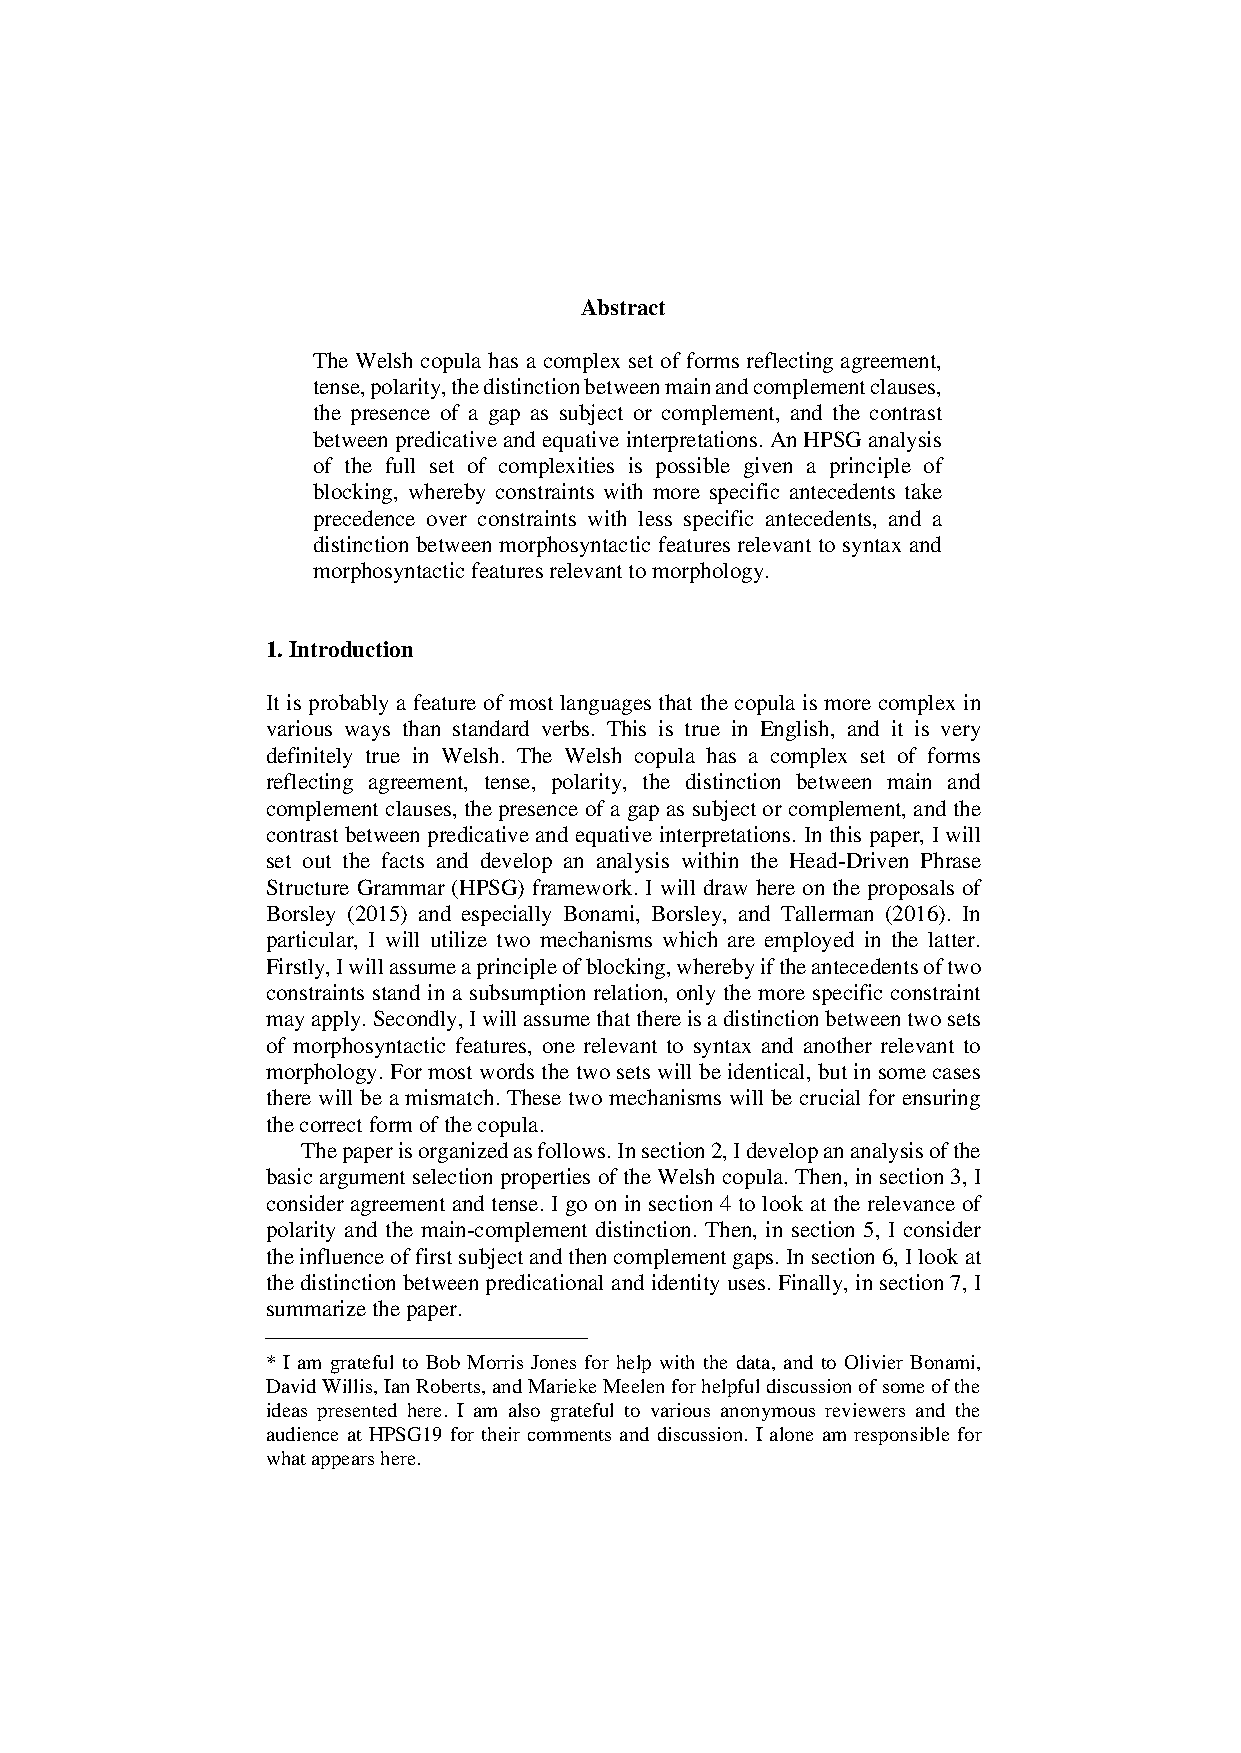
\includepdf[pages=-,pagecommand=\thispagestyle{plain}]{Includes/borsley.pdf}
        \setcounter{page}{26}
        \phantomsection
        \addcontentsline{toc}{section}{Matías Guzmán Naranjo: Analogy-based Morphology: The Kasem number system}
\thispagestyle{empty}

\begin{center}
  {\huge\bfseries Analogy-based Morphology: The Kasem number system\par}

  \bigskip

~\\
\begingroup
\setlength{\leftskip}{0pt plus 1fill}
\setlength{\rightskip}{0pt plus 1fill}
\setlength{\parindent}{0pt}
\setlength{\parfillskip}{0pt}
  \formatauthor{Matías Guzmán Naranjo}{\begin{tabular}{@{}c@{}}Université Paris Diderot\end{tabular}}

\par\endgroup

  \vspace*{8ex}

  Proceedings of the 26th International Conference on\par Head-Driven Phrase Structure Grammar

  \bigskip

  University of Bucharest

  \medskip

  Stefan  Müller, Petya Osenova (Editors)

  \medskip

  2019

  \medskip

  CSLI Publications

  \medskip

  pages 26--41

  \medskip

  \url{http://csli-publications.stanford.edu/HPSG/2019}
\end{center}
\vfill

\noindent



\vfill
\noindent
% APA Style
Guzmán Naranjo, Matías. 2019. Analogy-based Morphology: The Kasem number system. In Müller, Stefan, \& Osenova, Petya (Eds.), \emph{{Proceedings of the 26th International Conference on Head-Driven Phrase Structure Grammar, University of Bucharest}}, 26--41. Stanford,
CA: CSLI Publications. \hfill\href{http://creativecommons.org/licenses/by/4.0/}{
\includegraphics[height=.75em]{Includes/ccby-eps-converted-to.pdf}}

\newpage
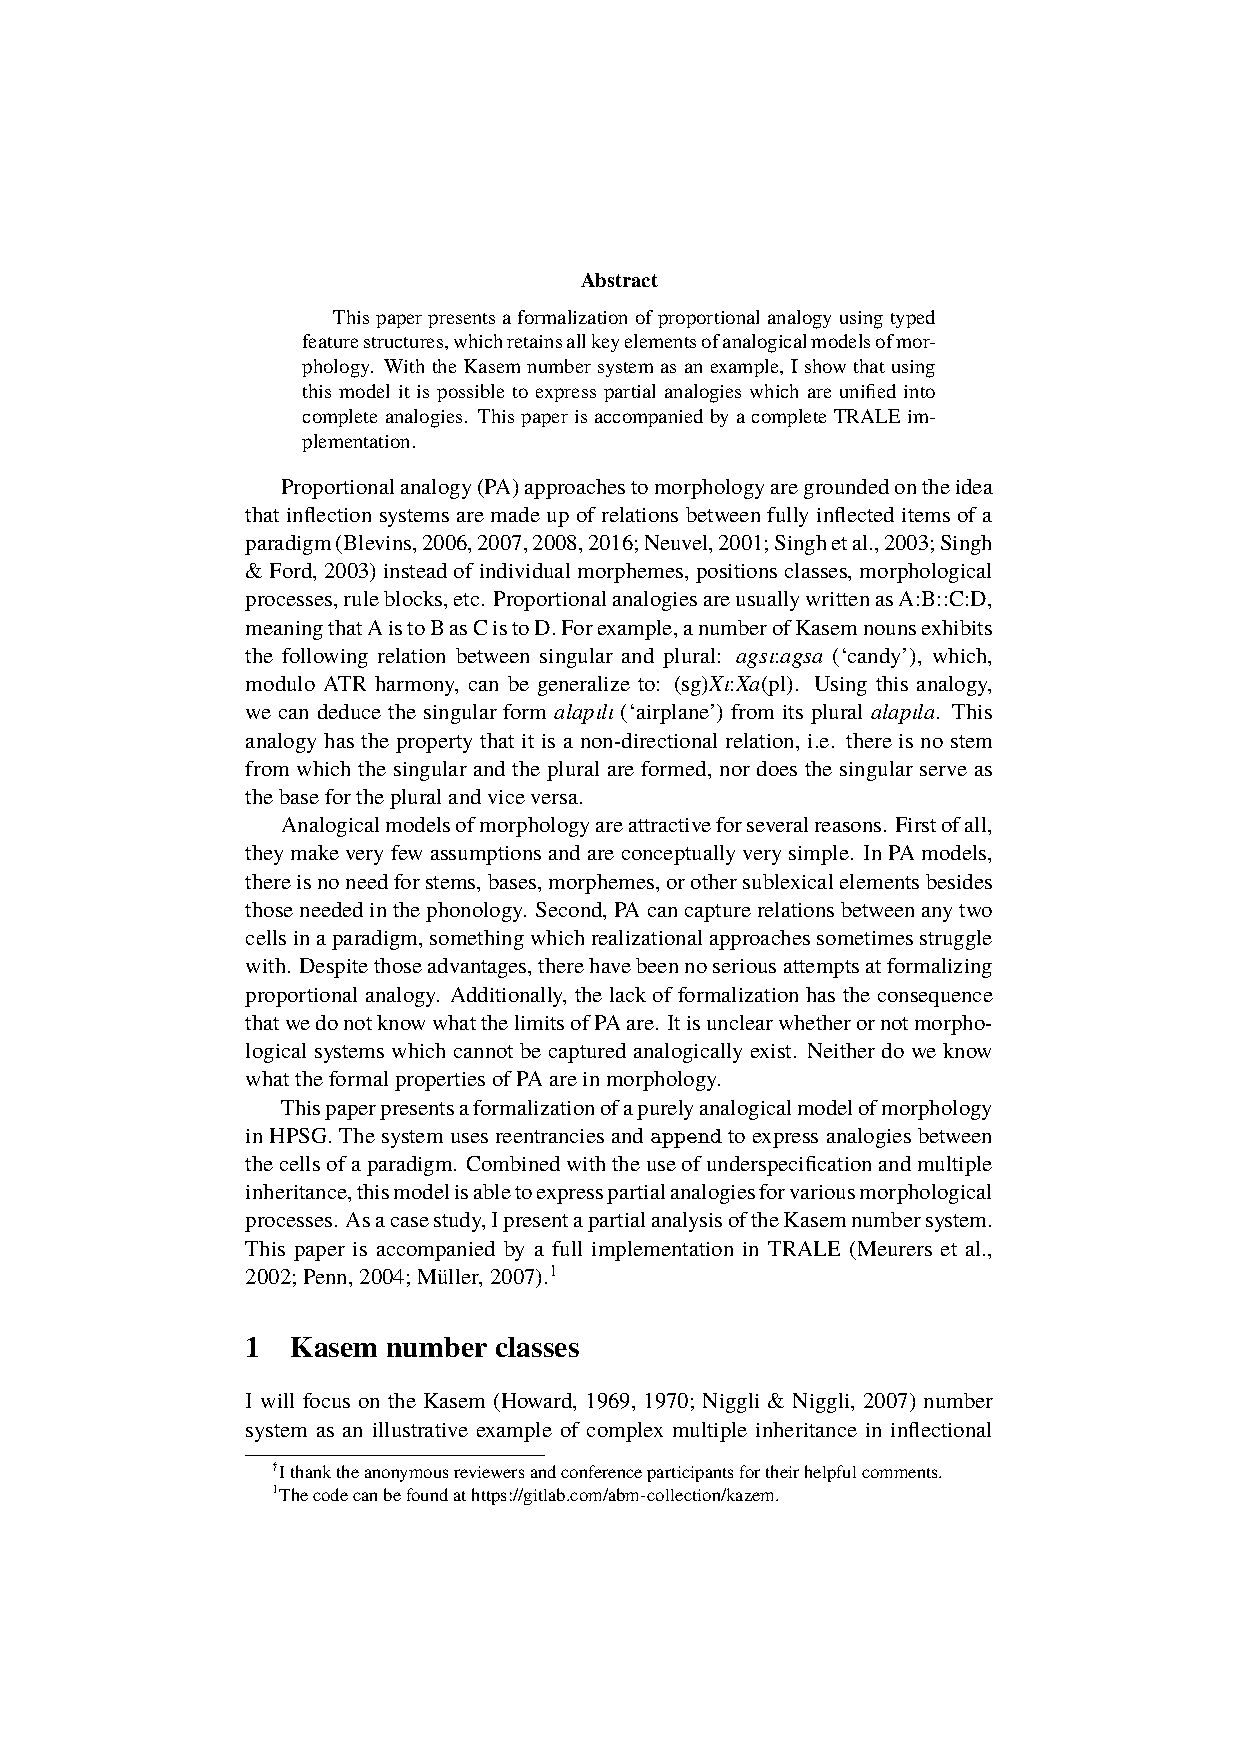
\includepdf[pages=-,pagecommand=\thispagestyle{plain}]{Includes/guzmannaranjo.pdf}
        \setcounter{page}{42}
        \phantomsection
        \addcontentsline{toc}{section}{Petter Haugereid: An incremental approach to gapping in Japanese}
\thispagestyle{empty}

\begin{center}
  {\huge\bfseries An incremental approach to gapping in Japanese\par}

  \bigskip

~\\
\begingroup
\setlength{\leftskip}{0pt plus 1fill}
\setlength{\rightskip}{0pt plus 1fill}
\setlength{\parindent}{0pt}
\setlength{\parfillskip}{0pt}
  \formatauthor{Petter Haugereid}{\begin{tabular}{@{}c@{}}Western Norway University of Applied Sciences\end{tabular}}

\par\endgroup

  \vspace*{8ex}

  Proceedings of the 26th International Conference on\par Head-Driven Phrase Structure Grammar

  \bigskip

  University of Bucharest

  \medskip

  Stefan  Müller, Petya Osenova (Editors)

  \medskip

  2019

  \medskip

  CSLI Publications

  \medskip

  pages 42--57

  \medskip

  \url{http://csli-publications.stanford.edu/HPSG/2019}
\end{center}
\vfill

\noindent
Keywords: HPSG, Gapping, Japanese, Incremental Parsing


\vfill
\noindent
% APA Style
Haugereid, Petter. 2019. An incremental approach to gapping in Japanese. In Müller, Stefan, \& Osenova, Petya (Eds.), \emph{{Proceedings of the 26th International Conference on Head-Driven Phrase Structure Grammar, University of Bucharest}}, 42--57. Stanford,
CA: CSLI Publications. \hfill\href{http://creativecommons.org/licenses/by/4.0/}{
\includegraphics[height=.75em]{Includes/ccby-eps-converted-to.pdf}}

\newpage
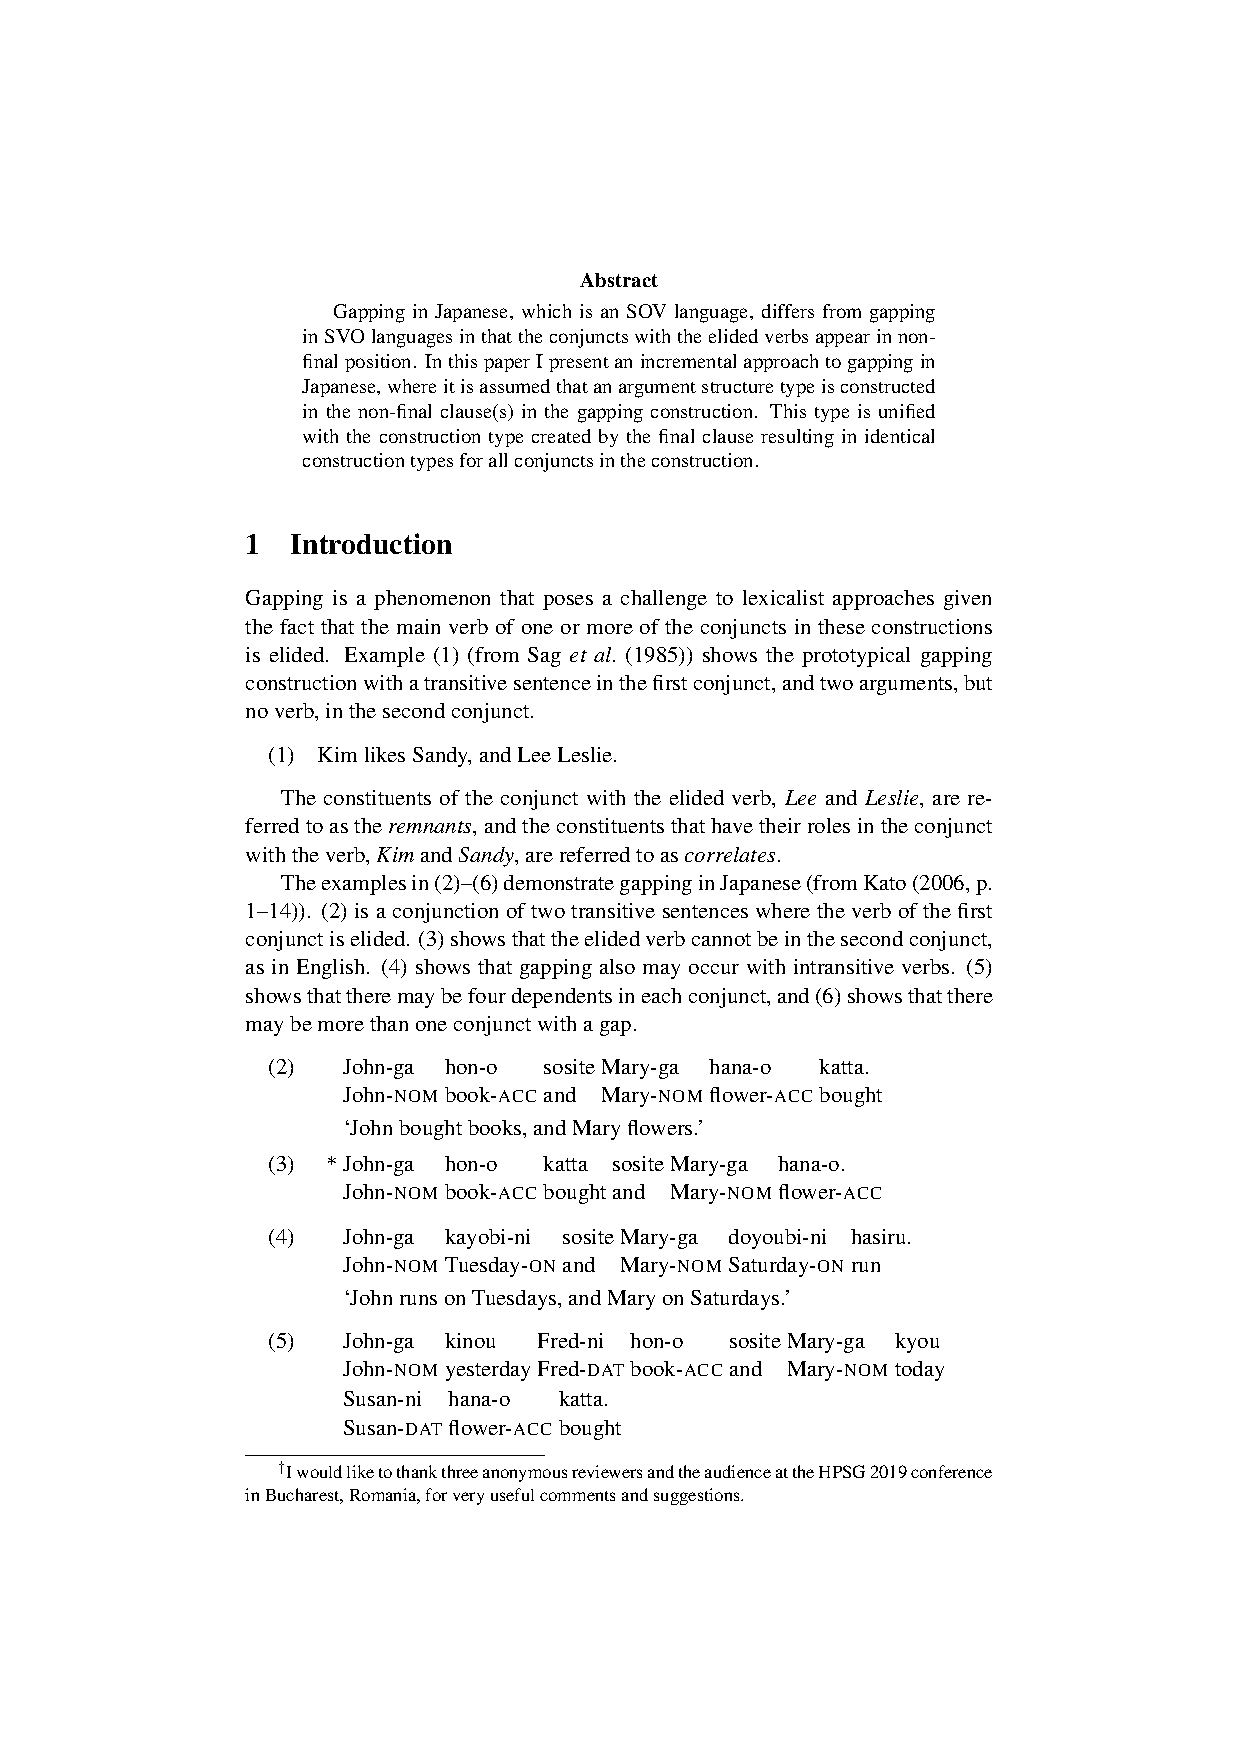
\includepdf[pages=-,pagecommand=\thispagestyle{plain}]{Includes/haugereid.pdf}
        \setcounter{page}{58}
        \phantomsection
        \addcontentsline{toc}{section}{Geoffrey K. Pullum: What grammars are, or ought to be}
\thispagestyle{empty}

\begin{center}
  {\huge\bfseries What grammars are, or ought to be\par}

  \bigskip

~\\
\begingroup
\setlength{\leftskip}{0pt plus 1fill}
\setlength{\rightskip}{0pt plus 1fill}
\setlength{\parindent}{0pt}
\setlength{\parfillskip}{0pt}
  \formatauthor{Geoffrey K. Pullum}{\begin{tabular}{@{}c@{}}University of Edinburgh\end{tabular}}

\par\endgroup

  \vspace*{8ex}

  Proceedings of the 26th International Conference on\par Head-Driven Phrase Structure Grammar

  \bigskip

  University of Bucharest

  \medskip

  Stefan  Müller, Petya Osenova (Editors)

  \medskip

  2019

  \medskip

  CSLI Publications

  \medskip

  pages 58--78

  \medskip

  \url{http://csli-publications.stanford.edu/HPSG/2019}
\end{center}
\vfill

\noindent
Keywords: grammars, HPSG, constraints, model-theoretic syntax


\vfill
\noindent
% APA Style
Pullum, Geoffrey K. 2019. What grammars are, or ought to be. In Müller, Stefan, \& Osenova, Petya (Eds.), \emph{{Proceedings of the 26th International Conference on Head-Driven Phrase Structure Grammar, University of Bucharest}}, 58--78. Stanford,
CA: CSLI Publications. \hfill\href{http://creativecommons.org/licenses/by/4.0/}{
\includegraphics[height=.75em]{Includes/ccby-eps-converted-to.pdf}}

\newpage
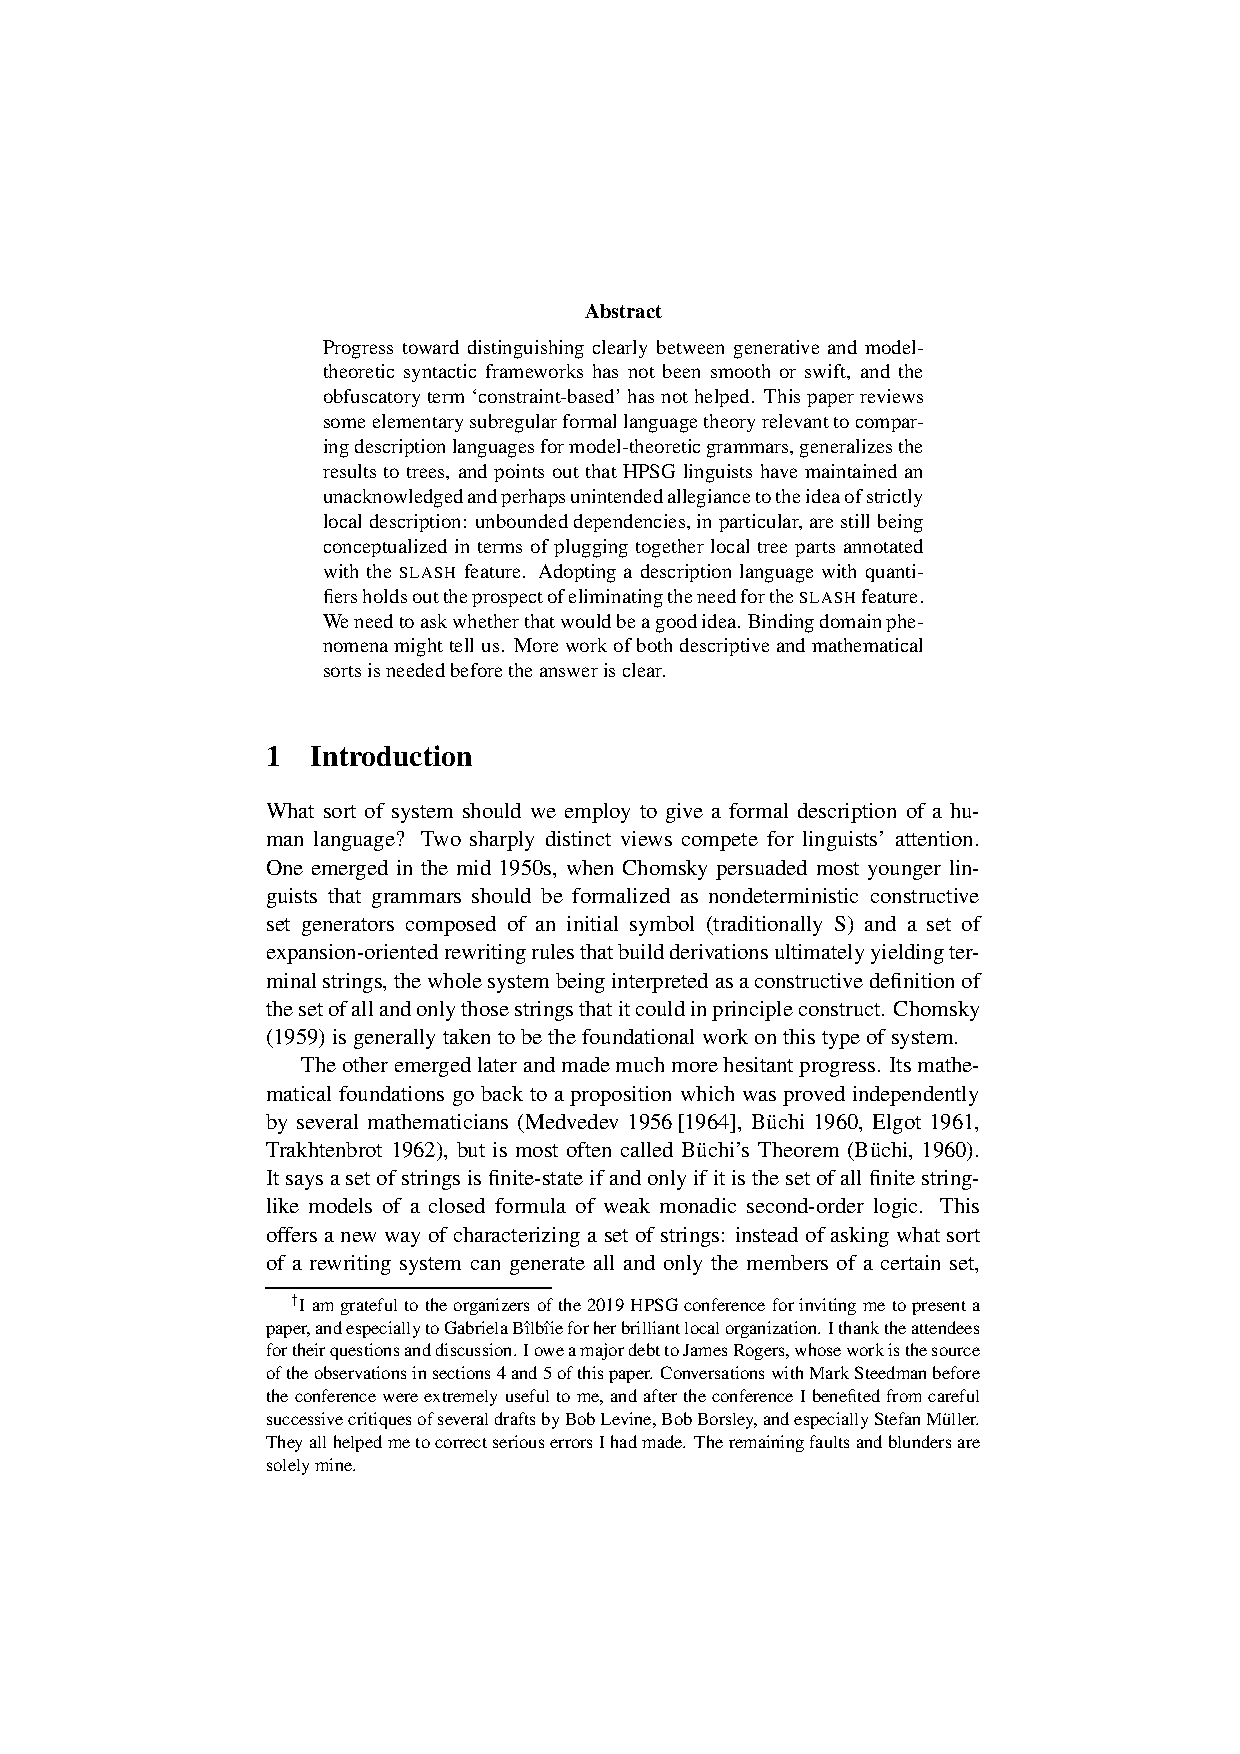
\includepdf[pages=-,pagecommand=\thispagestyle{plain}]{Includes/pullum.pdf}
        \setcounter{page}{79}
        \phantomsection
        \addcontentsline{toc}{section}{Monica-Mihaela Rizea, Manfred Sailer: Representing scales: Degree result clauses and emphatic
negative polarity items in Romanian}
\thispagestyle{empty}

\begin{center}
  {\huge\bfseries Representing scales: Degree result clauses and emphatic
negative polarity items in Romanian\par}

  \bigskip

~\\
\begingroup
\setlength{\leftskip}{0pt plus 1fill}
\setlength{\rightskip}{0pt plus 1fill}
\setlength{\parindent}{0pt}
\setlength{\parfillskip}{0pt}
  \formatauthor{Monica-Mihaela Rizea}{\begin{tabular}{@{}c@{}}Solomon Marcus Center for Computational Linguistics,
Bucharest\end{tabular}}
\formatauthor{Manfred Sailer}{\begin{tabular}{@{}c@{}}Goethe-University Frankfurt\end{tabular}}

\par\endgroup

  \vspace*{8ex}

  Proceedings of the 26th International Conference on\par Head-Driven Phrase Structure Grammar

  \bigskip

  University of Bucharest

  \medskip

  Stefan  Müller, Petya Osenova (Editors)

  \medskip

  2019

  \medskip

  CSLI Publications

  \medskip

  pages 79--99

  \medskip

  \url{http://csli-publications.stanford.edu/HPSG/2019}
\end{center}
\vfill

\noindent
Keywords: negative polarity item, result clause semantics, LRS, Romanian


\vfill
\noindent
% APA Style
Rizea, Monica-Mihaela, \& Sailer, Manfred. 2019. Representing scales: Degree result clauses and emphatic
negative polarity items in Romanian. In Müller, Stefan, \& Osenova, Petya (Eds.), \emph{{Proceedings of the 26th International Conference on Head-Driven Phrase Structure Grammar, University of Bucharest}}, 79--99. Stanford,
CA: CSLI Publications. \hfill\href{http://creativecommons.org/licenses/by/4.0/}{
\includegraphics[height=.75em]{Includes/ccby-eps-converted-to.pdf}}

\newpage
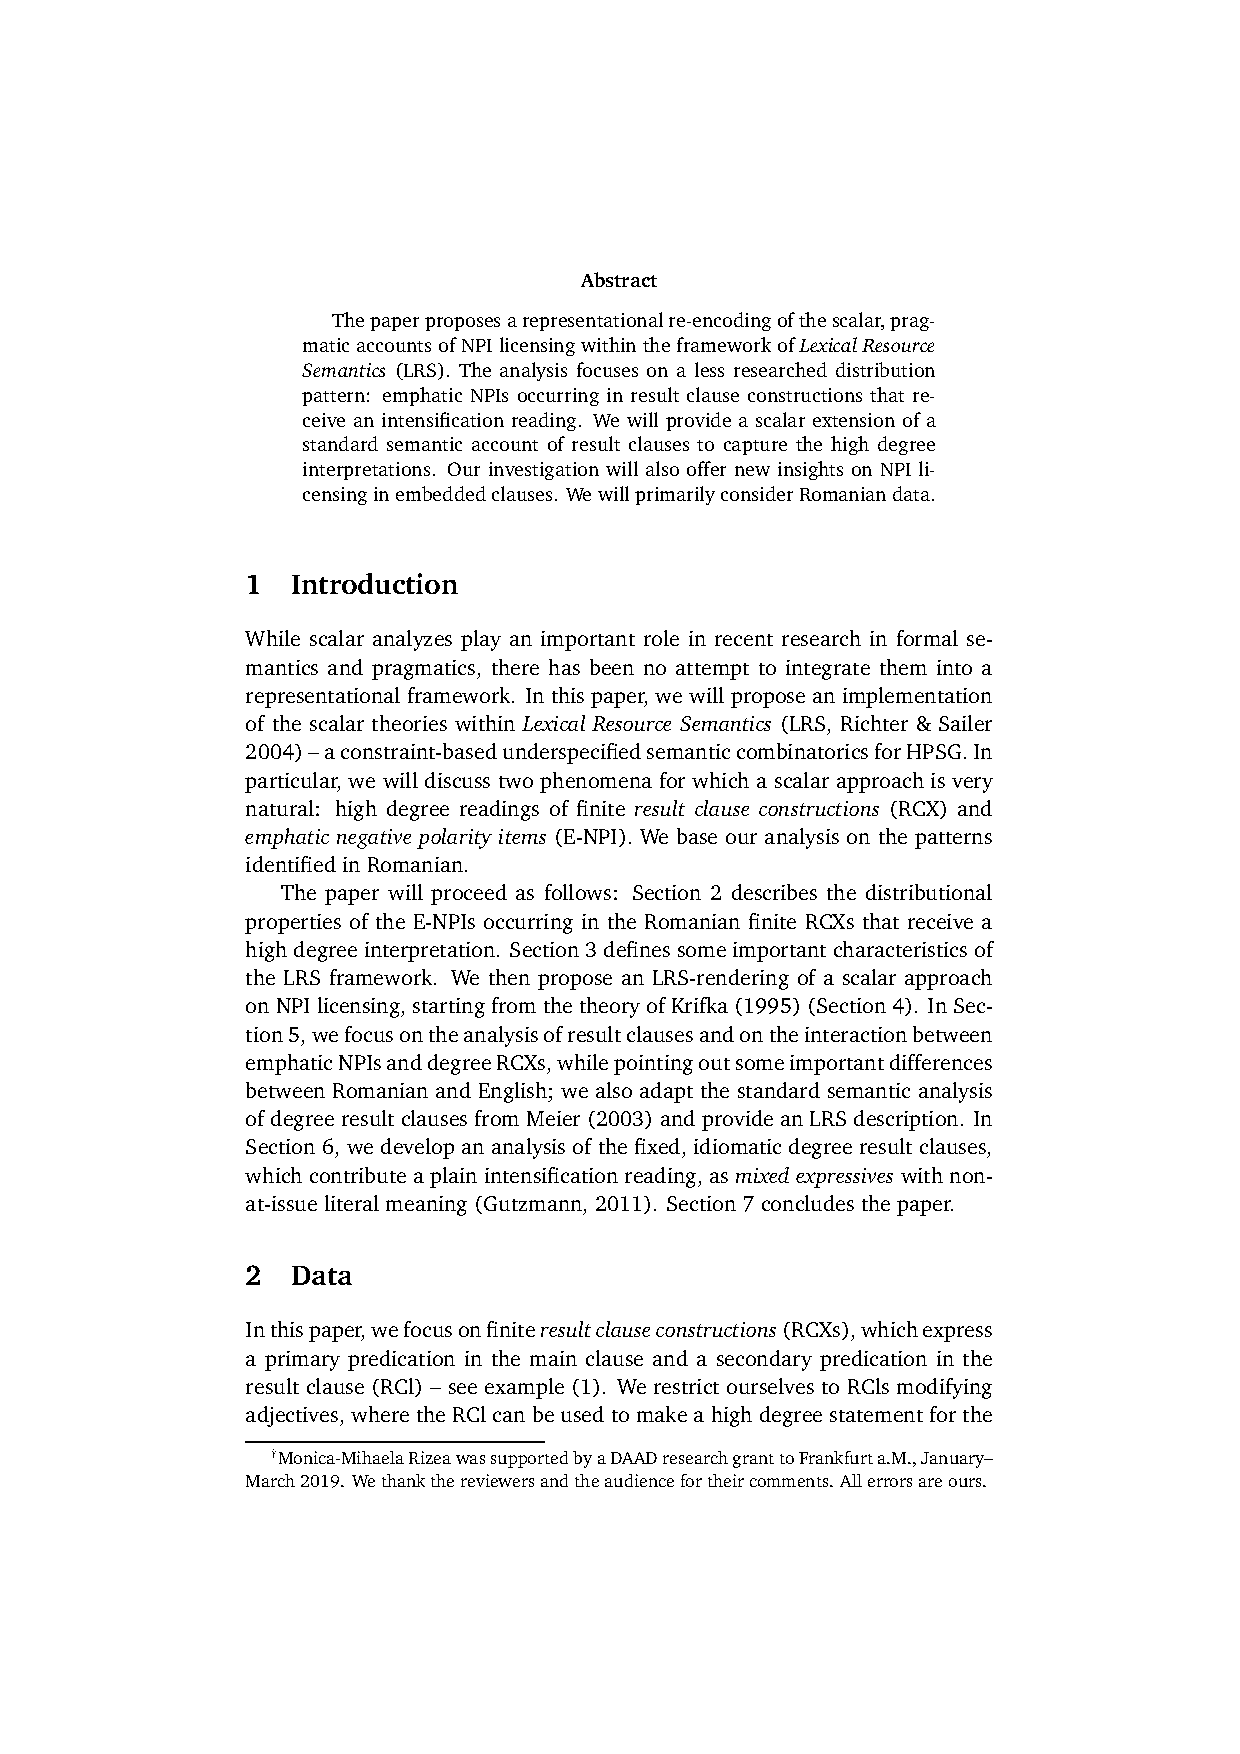
\includepdf[pages=-,pagecommand=\thispagestyle{plain}]{Includes/rizea-sailer.pdf}
        \setcounter{page}{100}
        \phantomsection
        \addcontentsline{toc}{section}{Gert Webelhuth, Olivier Bonami: Syntactic haplology and the Dutch proform "er"}
\thispagestyle{empty}

\begin{center}
  {\huge\bfseries Syntactic haplology and the Dutch proform "er"\par}

  \bigskip

~\\
\begingroup
\setlength{\leftskip}{0pt plus 1fill}
\setlength{\rightskip}{0pt plus 1fill}
\setlength{\parindent}{0pt}
\setlength{\parfillskip}{0pt}
  \formatauthor{Gert Webelhuth}{\begin{tabular}{@{}c@{}}University of Frankfurt\end{tabular}}
\formatauthor{Olivier Bonami}{\begin{tabular}{@{}c@{}}Universite de Paris, LLF, CNRS\end{tabular}}

\par\endgroup

  \vspace*{8ex}

  Proceedings of the 26th International Conference on\par Head-Driven Phrase Structure Grammar

  \bigskip

  University of Bucharest

  \medskip

  Stefan  Müller, Petya Osenova (Editors)

  \medskip

  2019

  \medskip

  CSLI Publications

  \medskip

  pages 100--119

  \medskip

  \url{http://csli-publications.stanford.edu/HPSG/2019}
\end{center}
\vfill

\noindent
Keywords: HPSG, Dutch, Haplology, ARG-ST, COMPS


\vfill
\noindent
% APA Style
Webelhuth, Gert, \& Bonami, Olivier. 2019. Syntactic haplology and the Dutch proform "er". In Müller, Stefan, \& Osenova, Petya (Eds.), \emph{{Proceedings of the 26th International Conference on Head-Driven Phrase Structure Grammar, University of Bucharest}}, 100--119. Stanford,
CA: CSLI Publications. \hfill\href{http://creativecommons.org/licenses/by/4.0/}{
\includegraphics[height=.75em]{Includes/ccby-eps-converted-to.pdf}}

\newpage
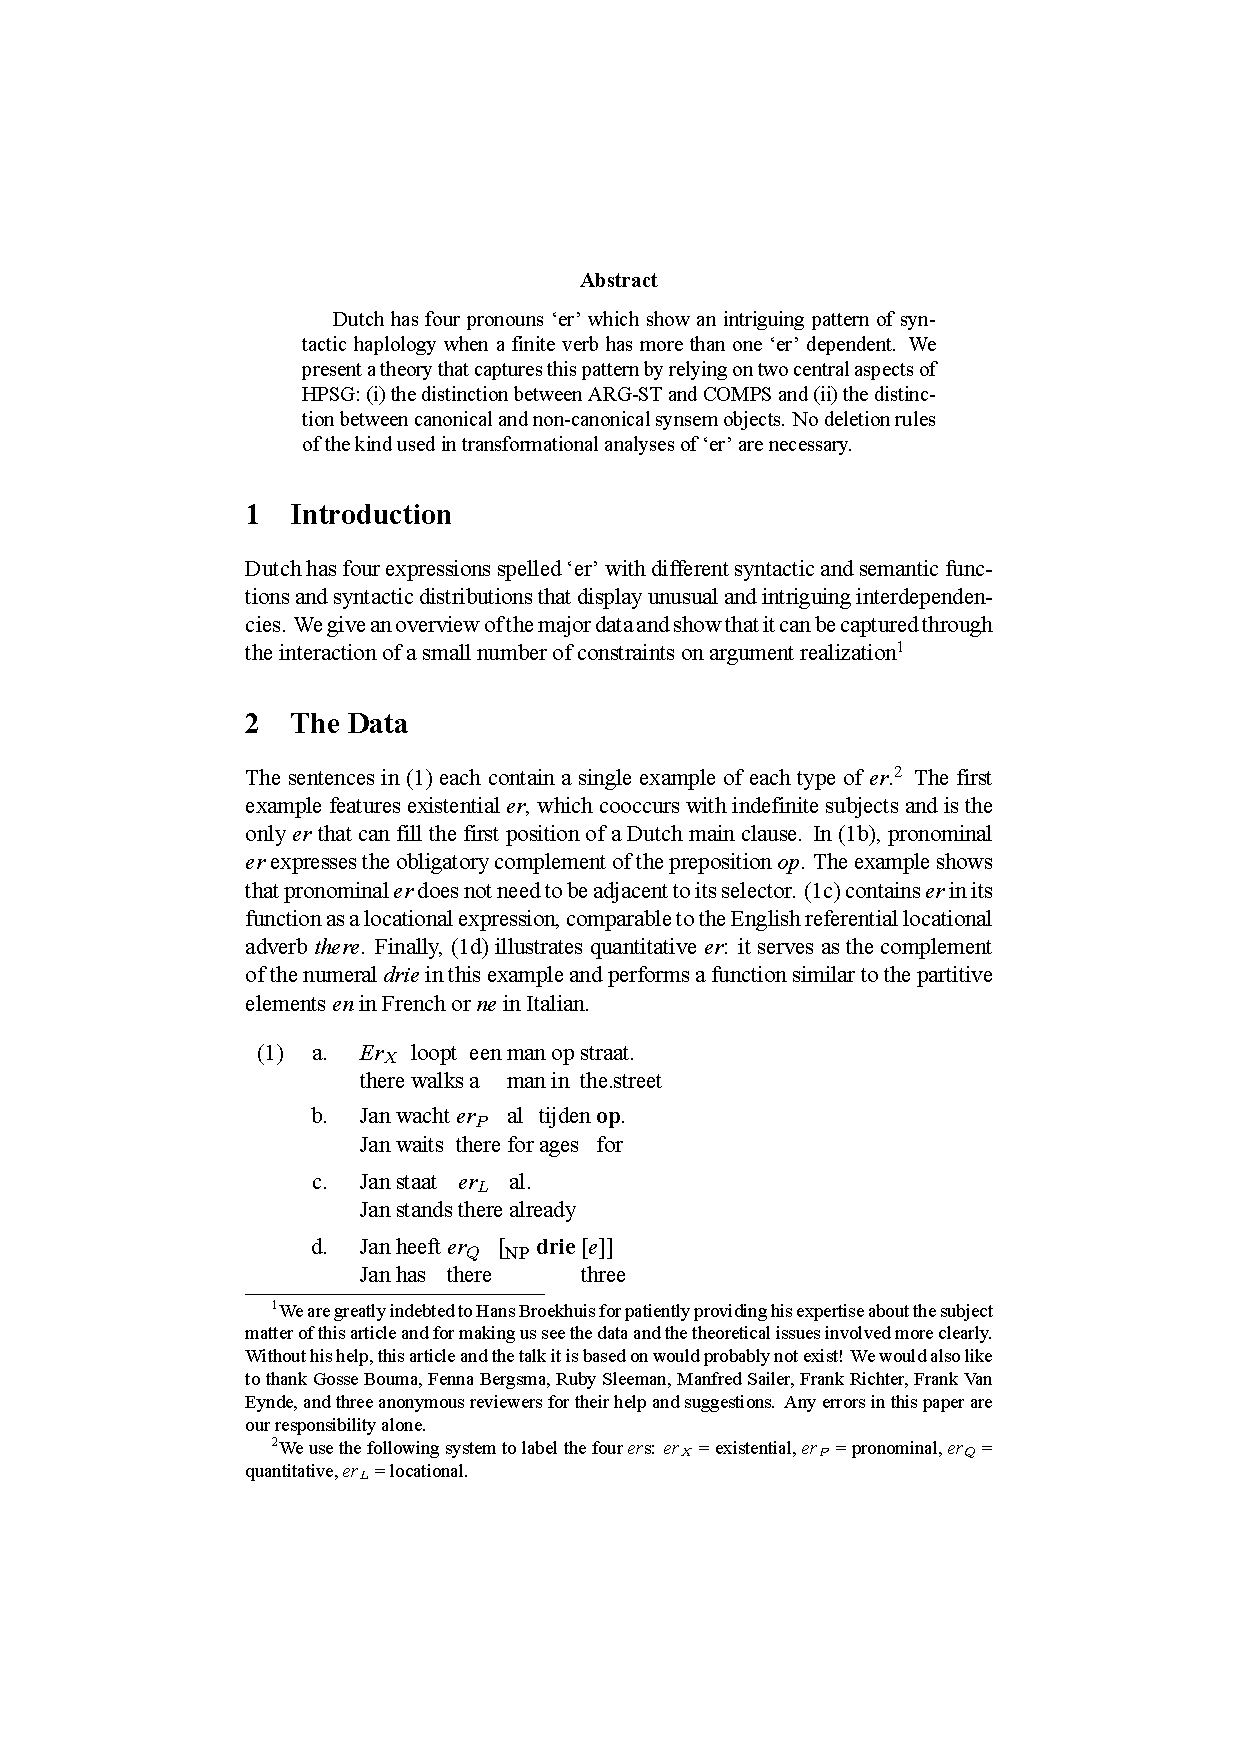
\includepdf[pages=-,pagecommand=\thispagestyle{plain}]{Includes/webelhuth-bonami.pdf}
\end{document}
